\section*{Постановка задачи}

\textbf{Задание:} используя хвостовую рекурсию, разработать, комментируя аргументы, эффективную программу, позволяющую:
\begin{enumerate}
	\item Сформировать список из элементов числового списка, больших заданного значения;
	\item Сформировать список из элементов, стоящих на нечетных позициях исходного списка (нумерация от 0):
	\item Удалить заданный элемент из списка (один или все вхождения);
	\item Преобразовать список в множество (можно использовать ранее разработанные процедуры).
\end{enumerate}

\begin{lstinputlisting}[label=third,caption=Решение задания №1, language=prolog, firstline=1, lastline=47]{../src/lab_18.pro}
\end{lstinputlisting}

\begin{figure}[H]
	\caption{Таблица к заданию.}
	\begin{center}
		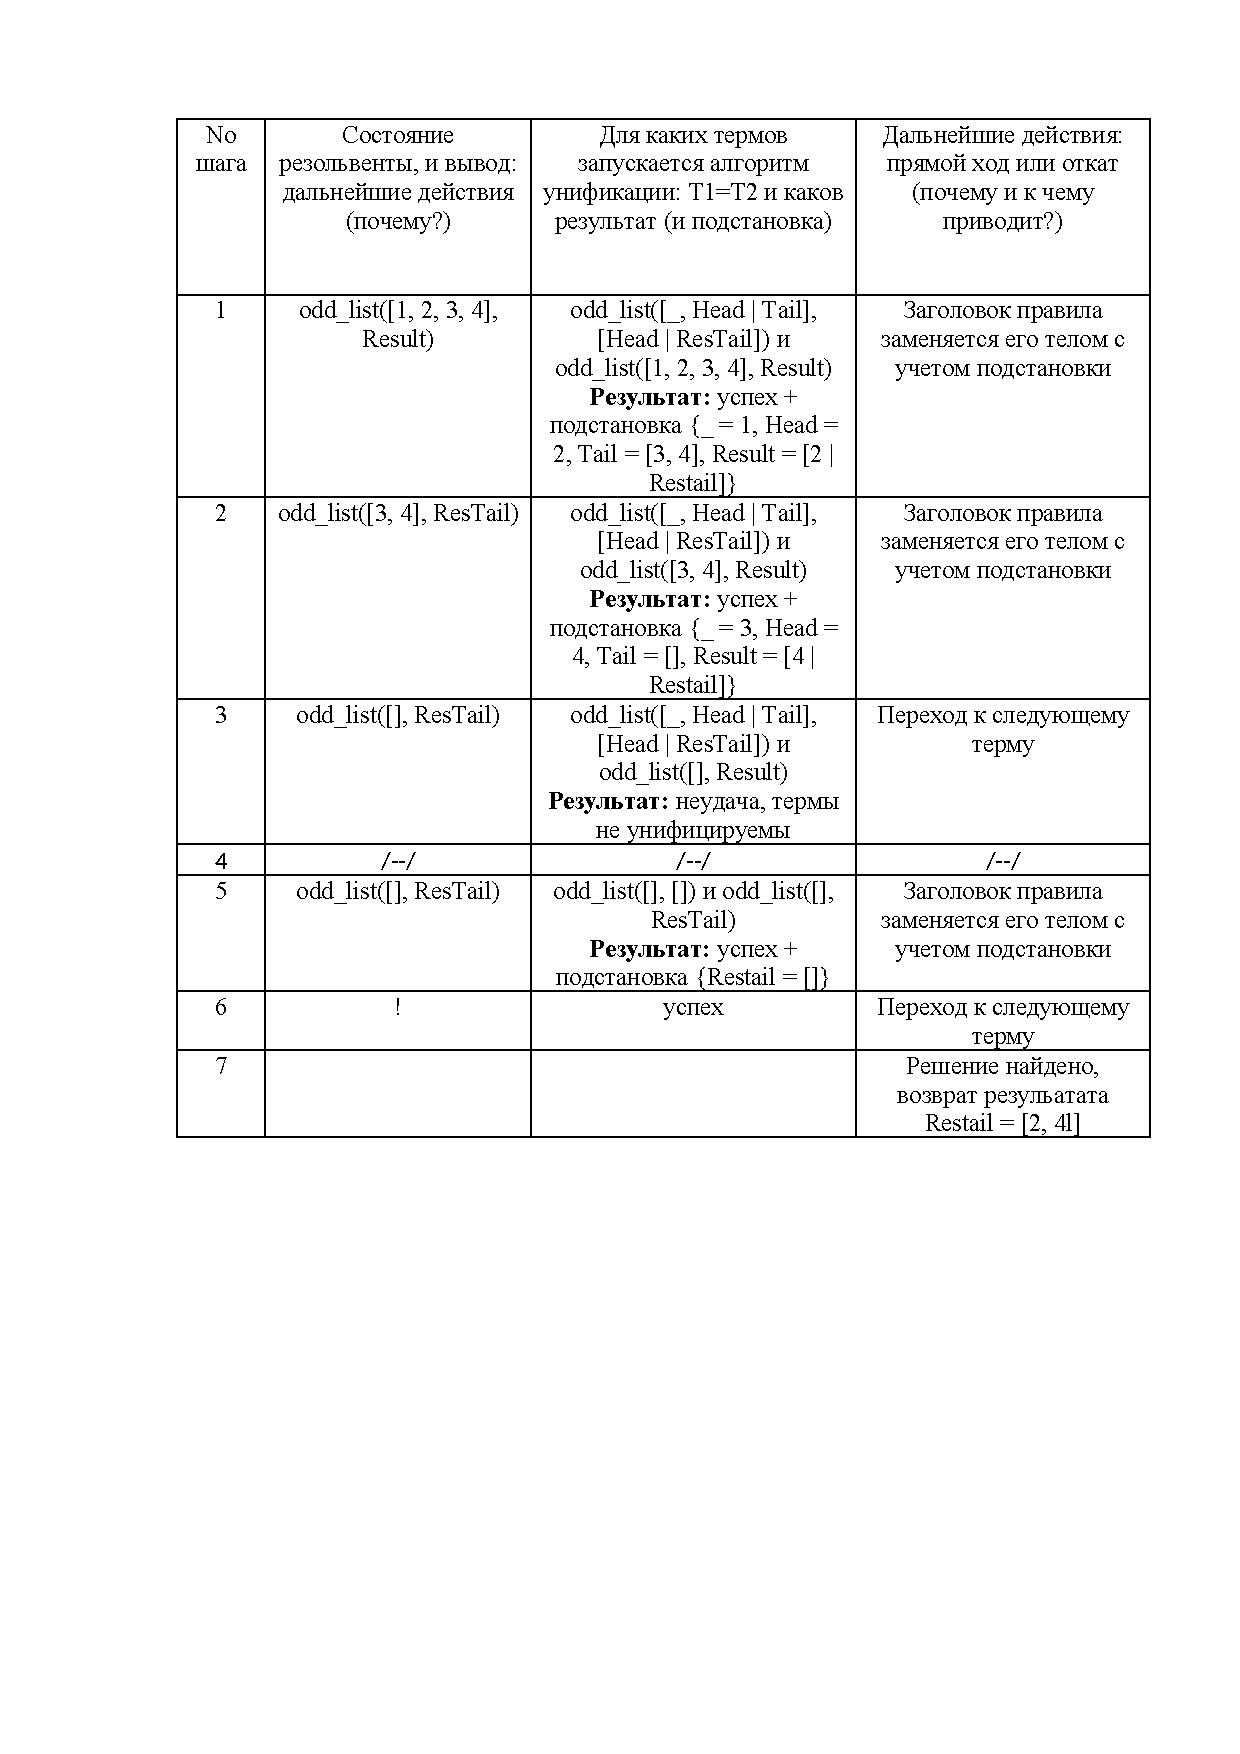
\includegraphics[scale=0.85]{img/18.1.pdf}
	\end{center}
	
\end{figure}
